% Derleme:  pdflatex teknik_rapor.tex  (iki kez, referanslar icin)
\documentclass[11pt,a4paper]{article}

\usepackage[utf8]{inputenc}
\usepackage[T1]{fontenc}
\usepackage[turkish,shorthands=off]{babel}
\usepackage{lmodern}
\usepackage[margin=2.4cm]{geometry}
\usepackage{amsmath,amssymb}
\usepackage{booktabs}
\usepackage{longtable}
\usepackage{array}
\usepackage{xcolor}
\usepackage{listings}
\usepackage{tikz}
\usetikzlibrary{shapes.geometric,arrows.meta,positioning,fit,backgrounds,calc}
\usepackage[hidelinks]{hyperref}

\definecolor{kod}{gray}{0.95}
\definecolor{iyi}{RGB}{0,110,60}
\definecolor{orta}{RGB}{175,110,0}
\definecolor{kotu}{RGB}{160,0,0}

\lstset{
  basicstyle=\ttfamily\footnotesize,
  backgroundcolor=\color{kod},
  frame=single, framerule=0pt,
  breaklines=true, columns=fullflexible,
  xleftmargin=4pt, xrightmargin=4pt,
  literate={ı}{{\i}}1 {İ}{{\.I}}1 {ş}{{\c s}}1 {Ş}{{\c S}}1
           {ğ}{{\u g}}1 {Ğ}{{\u G}}1 {ç}{{\c c}}1 {Ç}{{\c C}}1
           {ö}{{\"o}}1 {Ö}{{\"O}}1 {ü}{{\"u}}1 {Ü}{{\"U}}1
}

\newcommand{\yuksek}{\textcolor{iyi}{\textbf{Yüksek}}}
\newcommand{\bantli}{\textcolor{orta}{\textbf{Bantlı}}}
\newcommand{\disi}{\textcolor{kotu}{\textbf{Kapsam dışı}}}

\title{\textbf{CFD/FEA Analiz Paketi}\\[2mm]
\large Teknik Rapor: Yetenekler, Çalışma İlkesi ve Kullanım Alanları}
\author{}
\date{6 Ağustos 2026}

\begin{document}
\maketitle
\thispagestyle{empty}

\begin{abstract}
\noindent
Bu paket, katı modelden mühendislik hükmüne uzanan bütünleşik bir akışkanlar
(OpenFOAM) ve yapısal (CalculiX) analiz hattıdır. Ayırt edici özelliği çözücü
çeşitliliği değil, \emph{her sayının yanında ölçülmüş bir belirsizlik bandı ve
o bandın nereden geldiğini söyleyen bir gerekçe taşımasıdır}. Paket, savunulamaz
bir sonucu üretmeyi reddeder; reddederken nedenini ve düzeltme adımını yazar.
Kod tabanı 29.000 satır Python, 107 test dosyası ve 987 geçen testten oluşur.
Doğrulama zarfı 14 koşulda ölçülmüştür: analitik kapalı-formlara karşı yapısal
hata \%0--4.8, NASA Turbulence Modeling Resource'a karşı 2B profil sürüklemesi
GCI \%1.7, künt cisim sürüklemesi literatüre karşı \%6.0.
\end{abstract}

\vspace{4mm}

\section{Bu Paket Ne Yapar}

Üç soruyu yanıtlar:

\begin{enumerate}
  \item \textbf{Bu cisim havada/suda nasıl davranır?} Sürükleme, taşıma,
        moment, basınç dağılımı, ayrılma bölgeleri, sınır tabaka durumu.
  \item \textbf{Bu yapı bu yükü taşır mı?} Gerilme, deplasman, güvenlik
        faktörü, burkulma, modal frekans, termal gerilme.
  \item \textbf{Bu sayıya ne kadar güvenebilirim?} Ayrıklaştırma belirsizliği,
        model-form sapması, geçerlilik zarfı, ve sayının tasarım kararında
        kullanılıp kullanılamayacağı.
\end{enumerate}

Üçüncü soru, paketi tipik bir CFD sarmalayıcısından ayıran şeydir. Ticari ve
akademik yazılımların çoğu birinci ve ikinci soruyu yanıtlar; üçüncüsünü
kullanıcıya bırakır. Burada üçüncü soru \emph{kodun kendisinde} yaşar ve
yanıtı olumsuzsa sayı yayımlanmaz.

\section{Mimari}

\subsection{Katmanlar}

\begin{center}
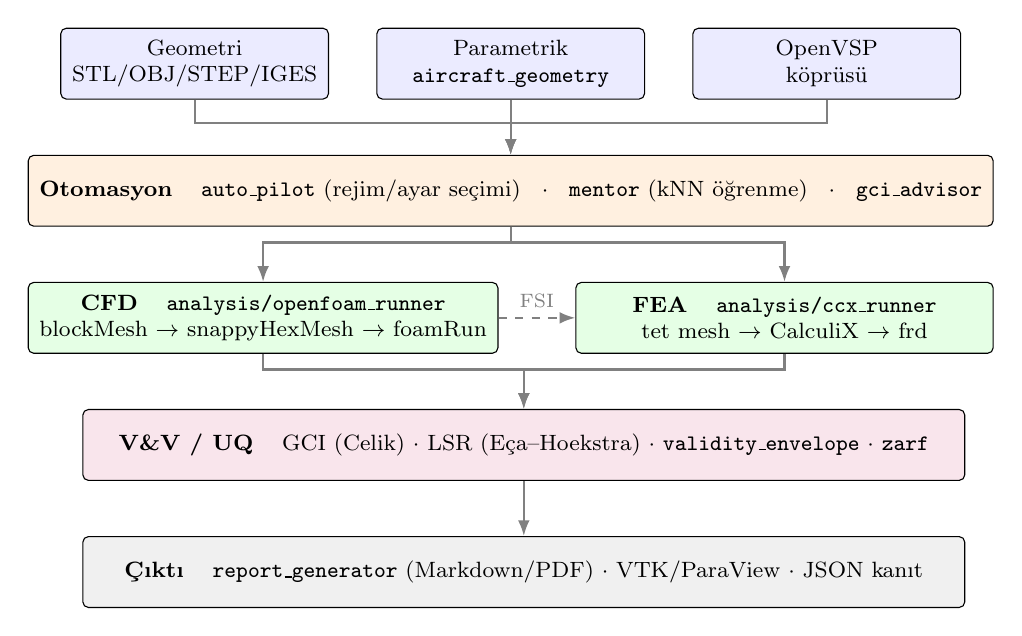
\begin{tikzpicture}[
  kutu/.style={draw, rounded corners=2pt, align=center, minimum height=9mm,
               font=\footnotesize, inner xsep=4pt},
  ok/.style={-{Latex[length=2mm]}, thick, gray}
]
\node[kutu, fill=blue!8, minimum width=34mm] (geo) {Geometri\\ STL/OBJ/STEP/IGES};
\node[kutu, fill=blue!8, minimum width=34mm, right=6mm of geo] (par) {Parametrik\\ \texttt{aircraft\_geometry}};
\node[kutu, fill=blue!8, minimum width=34mm, right=6mm of par] (vsp) {OpenVSP\\ köprüsü};

\node[kutu, fill=orange!12, minimum width=112mm, below=7mm of par] (oto)
  {\textbf{Otomasyon} \;\; \texttt{auto\_pilot} (rejim/ayar seçimi) \;\;$\cdot$\;\;
   \texttt{mentor} (kNN öğrenme) \;\;$\cdot$\;\; \texttt{gci\_advisor}};

\node[kutu, fill=green!10, minimum width=53mm, below=7mm of oto.south west, anchor=north west]
  (cfd) {\textbf{CFD} \;\; \texttt{analysis/openfoam\_runner}\\
         blockMesh $\rightarrow$ snappyHexMesh $\rightarrow$ foamRun};
\node[kutu, fill=green!10, minimum width=53mm, below=7mm of oto.south east, anchor=north east]
  (fea) {\textbf{FEA} \;\; \texttt{analysis/ccx\_runner}\\
         tet mesh $\rightarrow$ CalculiX $\rightarrow$ frd};

\node[kutu, fill=purple!10, minimum width=112mm, below=7mm of $(cfd.south)!0.5!(fea.south)$]
  (vv) {\textbf{V\&V / UQ} \;\; GCI (Celik) $\cdot$ LSR (Eça--Hoekstra) $\cdot$
        \texttt{validity\_envelope} $\cdot$ \texttt{zarf}};

\node[kutu, fill=gray!12, minimum width=112mm, below=7mm of vv] (rap)
  {\textbf{Çıktı} \;\; \texttt{report\_generator} (Markdown/PDF) $\cdot$ VTK/ParaView $\cdot$ JSON kanıt};

\draw[ok] (geo.south) -- ++(0,-3mm) -| (oto.north);
\draw[ok] (par.south) -- (oto.north);
\draw[ok] (vsp.south) -- ++(0,-3mm) -| (oto.north);
\draw[ok] (oto.south) -- ++(0,-2mm) -| (cfd.north);
\draw[ok] (oto.south) -- ++(0,-2mm) -| (fea.north);
\draw[ok] (cfd.south) -- ++(0,-2mm) -| (vv.north);
\draw[ok] (fea.south) -- ++(0,-2mm) -| (vv.north);
\draw[ok] (vv.south) -- (rap.north);
\draw[ok, dashed] (cfd.east) -- node[above, font=\scriptsize] {FSI} (fea.west);
\end{tikzpicture}
\end{center}

\subsection{Kanonik katman}

\texttt{analysis/} dizini ortak çekirdektir: \texttt{CFDCase} veri sınıfı, case
iskelesi kurulumu, mesh kalite kapısı, CalculiX yazıcı ve \texttt{.frd}
ayrıştırıcısı burada yaşar. Yeni CFD/FEA kodu bu katmanı kullanır; case
iskelesini yeniden yazmaz.

Depoda \emph{iki hızlı} bir durum vardır ve raporda gizlenmemelidir: eski
\texttt{simulation\_runner.py} ile bazı bağımsız V\&V betikleri bu katmanı
kullanmaz, kendi iskelesini tekrarlar. Bu bilinen bir teknik borçtur.

\section{Yetenekler}

\subsection{Akışkanlar (CFD)}

\begin{itemize}
  \item \textbf{Çözücü:} OpenFOAM 11, \texttt{foamRun}/\texttt{incompressibleFluid},
        kararlı-durum SIMPLE. Türbülans: $k$--$\omega$ SST (varsayılan),
        $k$--$\varepsilon$, ve geçiş modeli $k$--$\omega$ SST LM
        ($\gamma$--$\mathrm{Re}_{\theta}$).
  \item \textbf{Mesh:} \texttt{blockMesh} arka planı $+$ \texttt{snappyHexMesh}
        yüzey/kenar iyileştirmesi $+$ isteğe bağlı prizma katmanı. Arka plan
        hücresi \emph{bütçeden} boyutlandırılır (Bölüm~\ref{sec:kapilar}).
  \item \textbf{Araç hattı:} \texttt{vehicle\_pipeline} bir STL'den tam bir
        analiz üretir: tip önseti (uçak / roket / multikopter / araba / genel),
        far-field alanı, referans alanı, yakınsama izleme, y$^+$ ölçümü,
        mesh duyarlılık kampanyası ve mühendis raporu.
  \item \textbf{Polar taraması:} tek mesh üzerinde çoklu hücum açısı
        $\rightarrow$ $C_L$/$C_D$/$C_m$ eğrileri.
  \item \textbf{Panel/VLM yolu:} OpenVSP VSPAERO ile saniyeler mertebesinde
        taşıma eğimi ve panel yakınsaması; ince kanatta RANS'ın Kutta koşulunu
        kuramadığı durumlarda taşıma buradan alınır.
  \item \textbf{2B kesit:} XFOIL 6.99 sürücüsü (panel $+$ $e^N$ geçiş,
        $N_{\mathrm{krit}}=9$), panel-bağımsızlık ölçümü dâhil.
  \item \textbf{Aktüatör disk:} pervane itkisi kaynak terimi olarak.
\end{itemize}

\subsection{Yapısal (FEA)}

\begin{itemize}
  \item \textbf{Çözücü:} CalculiX, \texttt{.inp} formatı; üretim elemanı C3D10
        (kuadratik tetrahedron).
  \item \textbf{Yük mekanizmaları (beşi de doğrulanmış):} nokta/dağıtılmış
        kuvvet, basınç (tutarlı-yük: T6 yüzeyinde kenar-orta düğüme $A/3$),
        gövde kuvveti (yerçekimi / manevra $n\cdot g$), termal genleşme
        (\texttt{*EXPANSION}$+$\texttt{*TEMPERATURE}), ve burkulma (stabilite).
  \item \textbf{Malzeme veritabanı:} \texttt{materials.json} (10 malzeme),
        kaynaklı ve sürümlü.
  \item \textbf{Tekillik bekçisi:} keskin köşedeki sayısal tekilliği gerçek
        gerilme konsantrasyonundan ayırır; ayırmadan tepe gerilme raporlanmaz.
\end{itemize}

\subsection{Kuplaj ve optimizasyon}

\begin{itemize}
  \item \textbf{1-yönlü FSI:} CFD yüzey basıncı $\rightarrow$ FEA düğüm
        kuvvetleri. Korunum makine hassasiyetinde test edilir.
  \item \textbf{2-yönlü FSI:} Aitken ivmelendirmeli ilmek; aeroelastik
        ıraksama (divergence) tespiti.
  \item \textbf{Topoloji optimizasyonu:} SIMP, CFD-yüklü, gerilme kısıtlı
        (3B adjoint gerilme motoru sonlu-farkla doğrulanmış).
\end{itemize}

\subsection{Otomasyon ve öğrenme}

\begin{itemize}
  \item \texttt{auto\_pilot}: geometriden rejim, hız, mesh kalitesi, viskoz/
        inviscid seçimi ve referans alanını \emph{deterministik} olarak seçer;
        plan $+$ gerekçe döner, kullanıcı onaylar.
  \item \texttt{mentor}: geçmiş koşulardan kNN ile öğrenir. Öğrenme etiketi
        çözücünün çıkış kodu değil, \emph{geçerlilik kapısının hükmüdür} ---
        başarısız koşular negatif ders olarak kalır.
  \item \texttt{gci\_advisor}: yeni bir geometri için beklenen belirsizliği
        geçmiş kampanyalardan öngörür; bu öngörü UQ'ya \emph{girmez}, yalnız
        planlamaya yardım eder.
  \item \texttt{kanit}: her JSON kanıt dosyasının üretici komutunu denetler;
        yeniden üretilemeyen kanıtı işaretler.
\end{itemize}

\section{Nasıl Çalışır: Kapılar Mimarisi}
\label{sec:kapilar}

Paketin çekirdek fikri şudur: \emph{bir ölçüm, onu tüketen yere ulaşmıyorsa
yapılmamış sayılır.} Bu yüzden her aşamada, sonucu kesen kapılar vardır.
Kapılar koşudan \emph{önce} (bütçe koruması) ve \emph{sonra} (hüküm) çalışır.

\subsection{Koşudan önce}

\begin{itemize}
  \item \textbf{Arka plan bütçesi:} arka plan mesh'i hücre tavanının en fazla
        \%25'ini yiyebilir; aşarsa hücre \emph{kabalaştırılır}. Gerekçe
        ölçülmüştür: bu kapı yokken MiniHawk koşusunda 38{,}2$\times$22{,}5$\times$21{,}1~m
        alana serilen düzgün arka plan 3{,}94~M hücre üretiyor,
        \texttt{snappyHexMesh} 1{,}2~M'lik tavanı daha ilk adımda aşıyor ve
        \emph{hiçbir} yüzey iyileştirmesi yapamıyordu. Uçağın tamamı 74 yüzle
        temsil ediliyordu.
  \item \textbf{Yüzey çözünürlüğü ön-kapısı:} bir kademede gövdenin tahmini
        yüz sayısı 500'ün altına düşecekse o kademe \emph{koşulmaz}. Reddi
        koşudan sonra öğrenmek saatlerce CFD harcamak demektir.
  \item \textbf{İnce özellik hükmü:} firar kenarı gibi ince özelliklerin kaç
        hücreyle temsil edileceği önceden hesaplanır. Hedef $\geq 6$ hücredir;
        ulaşılamıyorsa taşımanın güvenilmez olacağı \emph{baştan} söylenir.
  \item \textbf{y$^+$ kademesi:} y$^+$'ı duvar-fonksiyonu bandına (30--300)
        sokan en ucuz iyileştirme kademesi geometri başına hesaplanır
        (\texttt{-{}-ref-bump oto}).
\end{itemize}

\subsection{Koşudan sonra}

\begin{itemize}
  \item \textbf{Yakınsama:} rezidüel eşiği \emph{tek başına} yeterli sayılmaz.
        Rezidüellerin platoya oturması (limit çevrimi) ile bütçenin bitmesi
        ayrıştırılır; ilki için ``daha çok iterasyon'' önerilmez, çünkü çözmez.
  \item \textbf{Fiziksel kabul:} negatif sürükleme, negatif indüklenen direnç,
        saçma $|C_L|$ gibi değerler kanıt dosyasına \emph{yazılamaz}.
  \item \textbf{Mesh kalitesi:} \texttt{maxNonOrthogonality} $<70$,
        \texttt{maxSkewness} $<4$.
  \item \textbf{Geçerlilik zarfı:} her büyüklük DOĞRULANMIŞ / EĞİLİM /
        ZARF-DIŞI olarak sınıflanır ve raporun en başına çocuk-okunur bir
        uyarı bloğu konur.
\end{itemize}

\subsection{Belirsizlik hiyerarşisi}

Ayrıklaştırma belirsizliği tek bir kaynaktan üretilir
(\texttt{band\_from\_levels}) ve kademe sayısına göre şu sırayla düşer:

\begin{center}
\begin{tabular}{@{}lll@{}}
\toprule
\textbf{Koşul} & \textbf{Yöntem} & \textbf{Kaynak} \\
\midrule
$n \geq 4$ kademe & En küçük kareler (LSR) & Eça \& Hoekstra 2014 \\
$n = 3$, monoton, $r \geq 1.3$ & Richardson $+$ GCI & Celik ve ark.\ 2008 \\
salınımlı & $U = 3\Delta_M$ & --- \\
$n = 2$ & vekil bant (bandın kendisi işaretli) & --- \\
\bottomrule
\end{tabular}
\end{center}

Temsili hücre boyu $h = N^{-1/d}$ ile hesaplanır ve $d$ \emph{çalışmanın
boyutudur}: hacim mesh'inde 3, 2B gridde 2, panel sayısında 1. Yanlış $d$
sessiz bir hatadır --- aynı veride $d{=}3$ ile $U=\%19{,}92$, $d{=}2$ ile
$U=\%9{,}80$ ölçülmüştür.

\subsection{Ayrıklaştırma ailesi kuralı}

Bir yakınsama bandı bir \emph{aile} için ölçülür. Üretim ayarı o ailenin bir
kademesi değilse band o sayıya ait değildir ve kapı devreye girer. Ayrıca aile
\emph{tek parametreli} olmalıdır: iki yönü aynı anda farklı oranlarda
değiştirmek Richardson'ın dayandığı varsayımı bozar.

Bu kuralın maliyeti ölçülmüştür. VLM panel çalışmasında yalnız açıklık yönü
inceltildiğinde (20$\rightarrow$120 panel) dizi yakınsama gösteremedi
($p<0{,}5$, $U=\%28{,}32$); çünkü sabit tutulan kiriş yönünün kendi gürültüsü
(\%1{,}9) açıklık adımlarından (\%0{,}5--1{,}2) büyüktü. İki yön birlikte
1{,}35 katıyla inceltilince ($40\times17 \rightarrow 98\times42$) dizi
monotonlaştı ve $U=\%1{,}36$'ya indi --- band 20{,}8 kat daraldı.

\section{Doğrulanmış Zarf}

Aşağıdaki tablo koddan üretilir (\texttt{python zarf.py}) ve README ile
senkron olduğu testle bağlanır. Her satır bir \emph{ölçüme} dayanır; ``beyan''
işaretli satırların kanıt dosyası yoktur ve öyle olduğu yazılıdır.

\begingroup
\footnotesize
\setlength{\tabcolsep}{4pt}
\begin{longtable}{@{}p{58mm}p{26mm}p{72mm}@{}}
\toprule
\textbf{Koşul} & \textbf{Güvenilirlik} & \textbf{Ölçülen kanıt} \\
\midrule
\endhead
2B profil mutlak $C_d$ ($M<0{,}3$, bağlı akış) & \yuksek &
NASA TMR NACA0012, $\alpha=0^\circ$: GCI \%1{,}7 ($p=0{,}666$); TMR sapması \%4{,}9 \\
\addlinespace
2B profil taşıma $C_l$ ($\alpha=8^\circ$) & \bantli &
En ince grid (917.504 hücre) $C_l=0{,}8556$ vs TMR $0{,}862 \rightarrow \%0{,}7$;
ancak 3-grid serisi ıraksıyor ($p=-2{,}463$), Richardson uygulanamadı \\
\addlinespace
Cilt sürtünmesi $C_f$ --- y$^+$ duyarlılığı & \yuksek &
Düz levha $\leftrightarrow$ Schlichting 1/7-kuvvet: ilk hücre $\leq\delta_{99}$
iken hata $\leq\%8$ (7 kademe); ilk hücre $3{,}0\,\delta_{99}$ olunca
(y$^+\approx864$) hata $-\%40$ \\
\addlinespace
3B künt cisim $C_d$ & \bantli &
Küp (Hoerner 1{,}05): $C_d=1{,}113$, sapma \%6{,}03; Richardson GCI \%3{,}1
($p=2{,}386$, asimptotik); 4-kademe LSR $U=\%58$ \\
\addlinespace
3B araç $C_d$ --- V\&V/UQ bandı & \bantli & Ölçülen validasyon bandı: bluff \%6{,}0 \\
\addlinespace
3B ince-kanatlı İHA --- araç hattı & \bantli &
MiniHawk (güncel): $C_d=0{,}0192$, gövde yüzeyi 24.477 yüz, y$^+_{\mathrm{ort}}=129$
(bant içinde). Mesh-bağımsızlık bandı YOK: ince kademe yakınsamadı
(rezidüeller platoda, limit çevrimi) \\
\addlinespace
Ayrılmış akış --- yeniden yapışma & \bantli &
Geriye-basamaklı akış $\leftrightarrow$ Driver \& Seegmiller 1985
($\mathrm{Re}_H=37500$): $X_r/H=5{,}54$ vs deney $6{,}26 \rightarrow -\%12$ \\
\addlinespace
Yapısal --- lineer statik (kiriş) & \yuksek &
Ankastre kiriş $\leftrightarrow$ Euler--Bernoulli: sehim \%1{,}0, gerilme \%3{,}9 \\
\addlinespace
Yapısal --- basınç yükü (hoop) & \yuksek &
İç-basınçlı silindir $\leftrightarrow$ Lamé: \%1{,}3 (T6 tutarlı-yük) \\
\addlinespace
Yapısal --- gerilme konsantrasyonu & \yuksek &
Delikli plaka $K_t \leftrightarrow$ Heywood: \%1{,}7 (C3D10, 6637 eleman) \\
\addlinespace
Yapısal --- termal gerilme & \yuksek &
Engellenmiş genleşme $\leftrightarrow \sigma=E\alpha\Delta T$: \%0{,}0 \\
\addlinespace
Yapısal --- burkulma & \yuksek &
Euler kolonu (ankastre-serbest, $K=2$): \%0{,}2 \\
\addlinespace
Yapısal --- öz-ağırlık & \yuksek &
Gövde kuvveti $\leftrightarrow \rho g L$: sehim \%0{,}2, gerilme \%4{,}8 \\
\addlinespace
Araç tipi sınıflandırma & \yuksek &
Tam kör üçüncü NX ailesi (27 geometri): preset doğruluğu \%96, kural tek
başına \%70 \\
\addlinespace
Stall / $C_{L,\max}$ & \bantli & Beyan: $\pm2$--$3^\circ$, $\pm\%15$ --- kanıt dosyası YOK \\
\addlinespace
y$^+<1$ duvar-çözünür geçiş & \disi & C-grid / DES gerekir \\
\bottomrule
\end{longtable}
\endgroup

\section{Bilinen Sınırlar}

Bunlar kusur değil, ölçülmüş kapsam sınırlarıdır; raporlarda da böyle görünür.

\begin{description}
  \item[İnce firar kenarı.] Bu donanımda (RTX 4060 sınıfı dizüstü) ince
        kanatlı bir İHA'nın firar kenarı 1--2 hücreyle temsil edilir. Kutta
        koşulu ağla kurulur; kurulamazsa sirkülasyon ve dolayısıyla
        \emph{taşıma} doğmaz. Ölçüldü: hücre sayısı 20{,}6 kat arttığında
        $C_l$ yalnız \%23 arttı. Hedef çözünürlük için yalnız yüzeyde
        $\sim775.000$ yüz gerekir. Bu yüzden ince kanatta taşıma VLM/panel
        yolundan, sürükleme ise birleştirmeden alınır.
  \item[Kararlı-RANS uygunluğu.] Bazı vakalarda rezidüeller platoya oturur ve
        kuvvetler limit çevrimine girer. Bu bir yakınsama eksikliği değil,
        akışın zaman-bağımlı olduğunun işaretidir; URANS gerekir.
  \item[Süpersonik mutlak $C_d$.] 3B-açık çözüm bu donanımda ulaşılamaz;
        eksenel-simetri/ince-cisim kuramıyla ele alınabilir rejim ayrıdır.
  \item[Panel yönteminin indüklenen direnci.] VSPAERO'nun iki $C_{Di}$ çıktısı
        da taşıyıcı-çizgi kuramından sapar (yakın-alan $-\%21$, Trefftz
        $+\%62$; Trefftz değeri sivriltilmiş kanatta $e>1$ ile Munk sınırını
        ihlal eder). Bu yüzden indüklenen direnç kuramdan üretilir; kuram
        eliptik planformda $e=1{,}00000$ vererek kendini doğrular.
  \item[Model-form belirsizliği.] Halen büyük ölçüde literatür-öncüldür
        (\%12 mertebesi); hat-özgü validasyon sürüyor.
\end{description}

\section{Nerelerde Kullanılabilir}

\subsection{Eğitim (BİLSEM ve dengi)}

Paketin \texttt{mentor} katmanı BYF/ÖYG/PROJE seviyelerine göre öğretici
kutular üretir ve geçerlilik banner'ı ``bu sayı tasarımda kullanılır mı''
sorusunu açıkça yanıtlar. Öğrencinin yanlış bir sayıyla roket/kanat
tasarlamasını engellemek açık bir tasarım hedefidir. Tipik kullanım: kanat
profili karşılaştırması, gövde biçimi--sürükleme ilişkisi, basit yapısal
kontrol.

\subsection{Yarışma takımları (TEKNOFEST vb.)}

Ön-tasarım döngüsü: STL $\rightarrow$ birkaç saatte $C_d$/$C_L$ bandı
$\rightarrow$ yapısal kontrol $\rightarrow$ rapor. Polar taraması ve aktüatör
disk desteği iticili konfigürasyonlar için yeterlidir. Önemli uyarı: ince
kanatta mutlak taşıma için VLM yolu kullanılmalıdır.

\subsection{Akademik çalışma}

Doğrulama çapaları (NASA TMR, Hoerner, Driver \& Seegmiller, Schlichting,
Lamé, Heywood, Euler) ve V\&V raporlama düzeni MDPI/IEEE beklentileriyle
uyumludur. GCI ve LSR bantları, kademe aileleri ve gözlenen mertebe $p$
doğrudan raporlanabilir biçimde saklanır. Her kanıt dosyası kendi üretim
komutunu taşır; \texttt{kanit.py} yeniden üretilemeyen kanıtı işaretler.

\subsection{Endüstriyel ön-tasarım}

Kavramsal aşamada eğilim analizi ve tasarım-alanı taraması için uygundur.
Sertifikasyon veya nihai tasarım doğrulaması için \emph{uygun değildir};
zarf tablosu hangi büyüklüğün hangi bantla geldiğini açıkça söyler.

\subsection{Uygun olmadığı yerler}

Duvar-çözünür geçiş ($y^+<1$) çalışmaları, yüksek Mach ayrılmalı akışlar,
çok-fazlı akış, yanma, ve zaman-çözünür aeroakustik bu paketin kapsamı
dışındadır.

\section{Kullanım}

\subsection{Kurulum}

\begin{lstlisting}
OpenFOAM 11        WSL2 (Ubuntu) uzerinde
CalculiX (ccx)     yerel ya da WSL
Python 3.13        numpy, scipy, trimesh, vtk, PyQt
opsiyonel          OpenVSP (conda ortami), XFOIL 6.99, gmsh
\end{lstlisting}

\subsection{Tipik komutlar}

\begin{lstlisting}
# Ana arayuz (arac analiz studyosu)
python app_analyzer.py

# Katti model -> CFD -> rapor, y+ kademesini otomatik sec
python vehicle_pipeline.py model.stl --tip ucak --hiz 15 \
       --kalite standart --ref-bump oto --duyarlilik --seviyeler 4

# Polar taramasi
python vehicle_polar.py model.stl --alfalar 0 4 8 12

# Yapisal kontrol (CFD basincindan)
python vehicle_fea.py --case vehicle_runs/model --malzeme AL6061

# Dogrulama zarfini yeniden uret
python zarf.py --yaz

# Kanit butunlugu denetimi
python kanit.py --eksik
\end{lstlisting}

\section{Kalite Güvencesi}

\begin{center}
\begin{tabular}{@{}lr@{}}
\toprule
Kod satırı (kök $+$ \texttt{analysis/}) & 29.023 \\
Kök modül & 76 \\
Deney/çapa betiği (\texttt{experiments/}) & 51 \\
Test dosyası & 107 \\
Geçen test & 987 \\
Atlanan test (harici bağımlılık/fixture) & 6 \\
\bottomrule
\end{tabular}
\end{center}

Testlerin ayırt edici yanı, \emph{sabit sonuç yerine niyet bağlamalarıdır}.
Örneğin bir test ``$C_d$ şu değere eşit olsun'' demez; ``rapor metni kendi
ölçtüğü seriyle çelişmesin'', ``ölçülmemiş bir band sıfır sayılmasın'',
``engel varsa mutlak sürükleme yayımlanmasın'' der. Böylece ölçüm değiştiğinde
test kırılmaz, ama \emph{tutarlılık} bozulduğunda kırılır.

\section{Sonuç}

Paketin değeri, ürettiği sayılardan çok \emph{üretmeyi reddettiği} sayılardadır.
Bir CFD koşusu her zaman bir sayı verir; o sayının anlamlı olup olmadığını
söylemek ayrı bir iştir ve bu paket o işi otomatikleştirir. Ölçülmüş
belirsizlik bandı, adı konmuş kapsam sınırı ve yeniden üretilebilir kanıt
dosyası; üçü bir arada olduğunda sonuç eğitimde güvenle, yarışmada hızla,
akademide savunulabilir biçimde kullanılabilir.

\end{document}
